\begin{figure}
	\tikzsetnextfilename{gauss-green-normale-y}
	\centering
	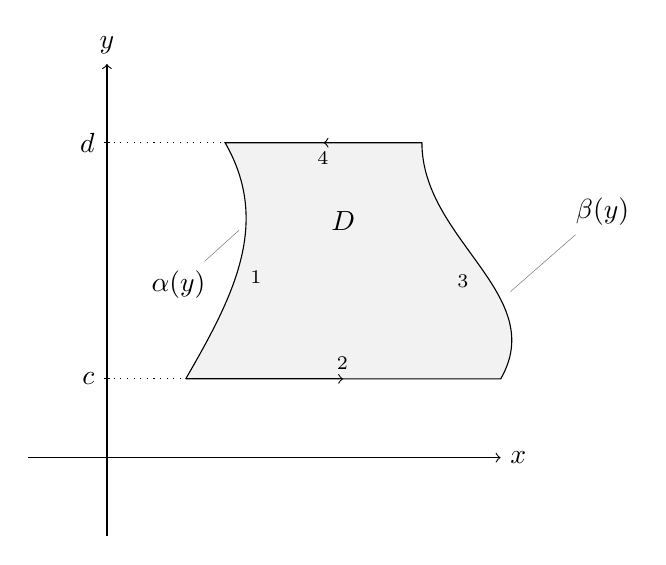
\begin{tikzpicture}
		\draw [black,->] (-1,0) -- (5,0) node[right]{$x$};
		\draw [black,->] (0,-1) -- (0,5) node[above]{$y$};
		\fill [black!5!white] (1,1) -- (5,1) to[out=60,in=270] (4,4) -- (1.5,4) to[out=300,in=60] (1,1);
		% \fill va prima del disegno del contorno, altrimenti si sovrappone a tutto e lo nasconde
		\draw [black] (1,1) to node[auto]{$\vgamma_2$} (5,1)
			to [out=60,in=270] node[auto]{$\vgamma_3$} (4,4)
			to node[auto]{$\vgamma_4$} (1.5,4)
			to [out=300,in=60] node[auto]{$\vgamma_1$} (1,1);
		\draw [dotted] (0,1) -- (1,1);
		\draw [dotted] (0,4) -- (1.5,4);
		\node [pin={[pin distance=5mm]230:{$\alpha(y)$}}] at (1.8,3) {};
		\node [pin={[pin distance=1cm]45:{$\beta(y)$}}] at (5,2) {};
		\node at (3,3) {$D$};
		% Dato che non TikZ non ha un comando per disegnare frecce in mezzo alla linea, mi devo arrangiare.
		% Traccio nuovamente le linee del bordo dell'insieme fino a -- più o meno -- metà, mettendo una freccia sulla
		% punta a queste. Non le disegno sui tratti curvi perche' sarebbe troppo complicato: dovrei spezzare in due anche
		% la linea tracciata prima con \draw (l. 10 e segg.) ma allora l'etichetta con il nome \vgamma del tratto non
		% risulterebbe più centrata.
		\draw [black,->] (1,1) -- (3,1);
		\draw [black,->] (4,4) -- (2.75,4);
		% Queste sono le tacche sull'asse y in corrispondenza delle due linee tratteggiate in y=c e y=d
		\draw (1pt,1) -- (-1pt,1) node[left]{$c$};
		\draw (1pt,4) -- (-1pt,4) node[left]{$d$};
	\end{tikzpicture}
	\caption{Parametrizzazione del contorno di un dominio $D$ come nel punto (i) della dimostrazione del teorema \ref{t:gauss-green} di Gauss-Green.}
	\label{fig:gauss-green-normale-y}
\end{figure}
